%!TEX root = ../rapport.tex

\chapter{Phase de tests production}
Cette phase finale sert à intégrer les résultats sur Thom, l'outils de supervision, ainsi que de tester le projet sur une situation équivalente à la production. Avoir un serveur avec une adresse publique, plusieurs Set-Top Box qui se connectent au serveur, ainsi qu'utiliser une ligne externe pour la connexion à Internet. Malheureusement cette phase de tests n'a pas pu être exécutée faute de temps.

\section{Thom}
Thom est donc l'outils de supervision de Wingo permettant d'accéder aux données des clients. Toutes les données permettant la supervision et le dépannage sont regroupées sur ce site. Voici la partie \textbf{IPTV} d'un client test.

\begin{figure}[H]
      \centering
      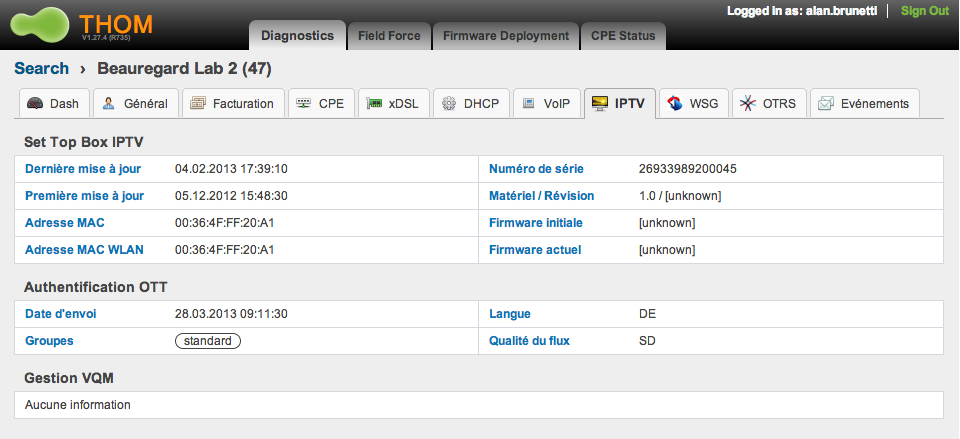
\includegraphics[width=\textwidth]{00_media/thom_iptv}
      \caption{Partie IPTV de Thom}
      \label{gra:maqmenu}
\end{figure}

Le but est de rajouter une partie \textbf{Remote Service} permettant de lancer les commandes sur la Set-Top Box via des boutons. Le résultat est le suivant:

\begin{figure}[H]
      \centering
      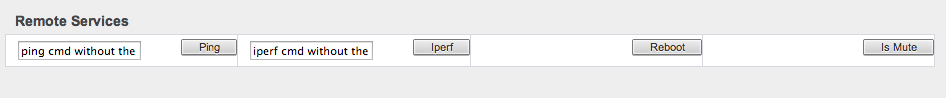
\includegraphics[width=\textwidth]{00_media/thom_remote}
      \caption{Ajout des boutons sur Thom}
      \label{gra:maqmenu}
\end{figure}

Nous voyons des inputs pour le ping et iperf permettant de mettre les options des commandes, alors que le reboot et isMute (que nous expliquerons au prochain chapitre) n'ont pas d'option.

\medskip

Lorsque la commande est lancée, le résultat s'affiche juste en dessous.
\begin{figure}[H]
      \centering
      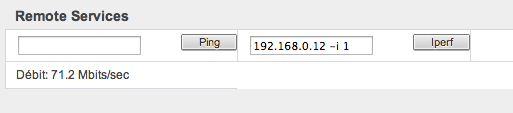
\includegraphics[width=200px]{00_media/thom_result}
      \caption{Résultat iperf sur Thom}
      \label{gra:maqmenu}
\end{figure}

\subsection{Conception}
Thom est réalisé en HTML, avec entre autre l'aide de Slimebone, une version personnalisée par Wingo de Backbone, un framework Javascript facilitant l'utilisation de Web Services et de la manipulation de données au format JSon.

Nous allons utiliser deux éléments de Backbone, les \textbf{views} et les \textbf{models}
\begin{itemize}
	\item \textbf{view}: Concerne tout ce qui est propre au HTML, la capture d'événements, la génération de code HTML dynamique
	\item \textbf{model}: Concerne la récupération de données sur un serveur à l'aide Web Service. Un model contient un paramètre URL qui est l'URL du Web Service auquel nous voulons accéder.
\end{itemize}

J'utilise 4 views et 4 models, chacun pour un service proposé. Nous allons nous concentrer sur Iperf, puis que le reste est identique au niveau de l'utilisation.

\medskip

La view \textbf{Thom.Views.Stbs.Iperf} est la vue qui donc propre à Iperf. Elle réagira au clique sur le bouton correspondant, et appellera le model \textbf{Thom.Models.Stb} pour que lui aille chercher les données sur le serveur.

\begin{figure}[H]
      \centering
      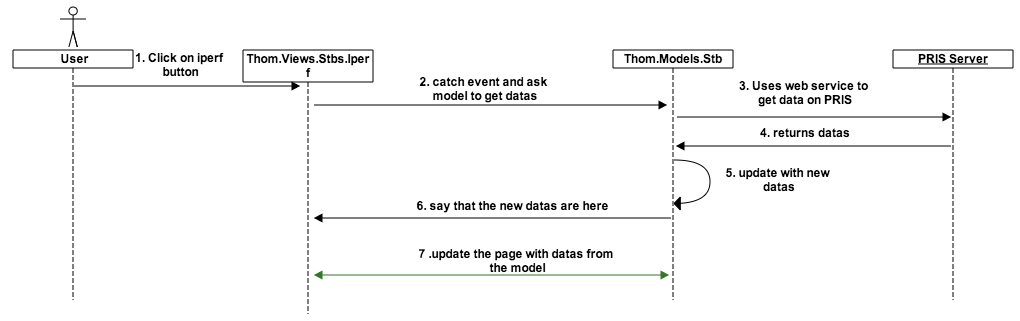
\includegraphics[width=\textwidth]{00_media/backbone_working}
      \caption{Fonctionnement de Backbone}
      \label{gra:maqmenu}
\end{figure}

\subsection{Implémentation}
\subsection{HTML de base}
Ici, nous allons créer une nouvelle table HTML contenant les nos 4 boutons. Ceci est fait de manière statique, mais l'on pourrait tout à fait imaginer un Web Service nous retournant les commandes disponibles dans le futur!
\begin{lstlisting}[language=HTML, caption={Table HTLM}]
<table class='diagnostics vertical' id='qos_result'>
	<caption>Remote Services</caption>
	<tr>
		<th><input type='text' id='ping_input' value='ping cmd without the ping'/><a class='button' id='btn_ping' href='javascript:void(0);'>Ping</a></th>
		<th><input type='text' id='iperf_input' value='iperf cmd without the iperf'/><a class='button' id='btn_iperf' href='javascript:void(0);'>Iperf</a></th>
		<th><a class='button' id='btn_reboot' href='javascript:void(0);'>Reboot</a></th>
		<th><intput type='text' id='isMute_cell' disable/><a class='button' id='btn_isMute' href='javascript:void(0);'>Is Mute</a></th>
	</tr>
</table>
\end{lstlisting}

Ce qui est important, ce sont sont les IDs. En effet, avec jQuery, nous pouvons facilement interagir avec le HTML en se basant sur l'ID des éléments, et Backbone aussi! Par exemple, nous voyons que le clique sur un bouton ne fait rien, mais c'est la View qui va intercepter l'événement et le traiter.

\medskip

Donc l'ID de la table est \textbf{qos\_result}, l'ID du bouton est \textbf{btn\_iperf} et l'ID du input est \textbf{iperf\_input}.
\subsubsection{Initialisation}
Premièrement, il faut récupérer la valeur de la MAC adresse stockée dans la cellule dont l'ID est \textbf{stb\_mac\_addr}.

Ensuite, il faut instancier un Model pour Iperf, ainsi qu'une View. On passera en paramètre le Model à la View.

Tout ceci se fait dans la page HTML. Le script se lancera automatiquement au chargement de la page.

\begin{lstlisting}[language=HTML, caption={Initialisation du Model et de la Vue}]
<script type="text/javascript">
	 $(function() {
	 	var macAddr = $('#stb_mac_addr').text();
	 	var iperfModel = new Thom.Models.Stb({path:'iperf/'+macAddr});
    	new Thom.Views.Stbs.Iperf({model:iperfModel});
  });
</script>
\end{lstlisting}

Le paramètre \textbf{path} est le chemin relatif du Web Service par rapport à \textbf{http://server\_adresse/qosServer/rest/stb}

\subsubsection{View}
Nous allons voir quel est le code derrière une View. Nous allons voir que cela fonctionne de manière clé/valeur, à savoir que l'on peut déclarer par exemple une fonction, dont le nom sera la clé, et la valeur sera l'implémentation de la fonction.
\begin{lstlisting}[caption={Code de la View}]
Thom.Views.Stbs.Iperf = Slimbone.View.extend({
	el: 'table#qos_result',

	initialize: function(){
		this.$list = this.$el.find("tbody:last");
		this.model.on('fetch:success'   , this.renderSuccess   , this);
	},

	events: {
		'click #btn_iperf': 'fetch'
	},

	fetch: function(){
		var value = $('#iperf_input').val();
		this.model.opt = value;
		this.model.cmd = 'iperf';
		this.model.fetch({
			success:this.renderSuccess
		});

	},
	cleanList: function() {
    	this.$list.children().not("tr:first").remove();
  	},
	renderSuccess:function(){
		console.log('fetch success');
		console.log(this.model);
		var values = this.model.val;
		this.cleanList();
        this.$list.append(
          '<tr>' +
		 '<td> Debit: ' + values.throughput + ' '+values.unit+'</td>' +
		 '</tr>'
        );
	}
});
\end{lstlisting}

\begin{table}[H]
\begin{tabularx}{\textwidth}{|m{3cm}|X|l|}
  \hline
  \bf{Clé} & \bf{Description} \\
  \hline
  el & L'élément el est le tronçon HTML dont la View peut avoir accès. Cela veut dire que la View ne peut pas manipuler tous les éléments parents de el, mais les enfants oui. Nous lui donnons ici la table qos\_result, dont on pourra donc manipuler tout le contenu.\\
  \hline  
  initialize & Méthode appelée en tout premier lorsque l'on instancie la View. Il s'agit en quelque sorte d'un constructeur. Nous l'utilisons ici pour définir une variable \textbf{list}, qui est la fin de notre table HTML, puis nous disons d'appeler la méthode \textbf{fetch\_success}lorsque le Model a correctement été chercher les données sur le serveur.\\
  \hline  
  events & Permet d'interagir avec les événements produits par l'utilisateur. Ici, lorsque l'événement \textbf{click} intervient sur le bouton \textbf{btn\_iperf}, on lance la méthode fetch.\\
  \hline  
  fetch & Fetch veut dire "aller chercher". Lorsque l'utilisateur à fait un click, nous allons dire au Model d'aller chercher les données. Nous en profitons pour lui changer ses paramètres: on récupère les options écrites dans le input \textbf{iperf\_input} et on lui précise que la commande sera bien un \textbf{iperf}, en vue de construire le Json envoyé au serveur.\\
  \hline  
  cleanList & Permet de vide la table d'ancien résultat pour afficher par la suite les nouveaux.\\
  \hline 
  renderSuccess & Lorsque le Model a fini de récupérer les données, cette méthode est appelée. On peut maintenant ajouter du contenu HTML avec les valeurs que le Model a récupérées sur le serveur.
 \end{tabularx}
\caption{Résumé d'une View}
\label{tab:classDiagram}
\end{table}

\subsubsection{Model}
Même principe ici. Sauf que nous n'avons pas un Model propre à chaque commande, mais un seul que nous personnalisons grâce aux paramètres différents qu'il prendra.

\begin{lstlisting}[caption={Code du Model}]
		Thom.Models.Stb = Slimbone.Model.extend({
			
			initialize: function(attributes) {
      			this.path = attributes.path;
      			this.opt = null;
      			this.cmd = null;
      			_.bindAll(this);
    		},
			fetch: function(){

				if(this.opt!==null){
					this.jsonopt = "{\"opt\":\""+this.opt+"\",\"cmd\":\""+this.cmd+"\"}";
					this.finalPath = 'http://localhost:8080/qosServer/rest/stb/'+this.path+'?cmd='+this.jsonopt;
				}
				else{
					this.finalPath = 'http://server:8080/qosServer/rest/stb/'+this.path;
				}
				console.log('fetching to :'+this.finalPath);
				Slimbone.ajax({
					url:this.finalPath,
					dataType: 'json',
					success: this.commandSuccess,
					error: this.commandError
				});
			},
			commandSuccess: function(resp) {
				this.val = resp;
				this.trigger('fetch:success');
			},

			commandError: function(jqXHR, textStatus, errorThrown) {
   	 			console.log(textStatus);
  			}
		});
\end{lstlisting}
\begin{table}[H]
\begin{tabularx}{\textwidth}{|m{3cm}|X|l|}
  \hline
  \bf{Clé} & \bf{Description} \\
  \hline
  initialize & Comme pour la View, cette méthode permet d'initialiser le Model avec certains attributs. Dans notre cas, lors de sa création nous lui avions passé un paramètre \textbf{path} que pouvons ici récupérer. Ensuite, nous déclarons deux autres attributs: \textbf{opt}, le contenu de l'input mis à disposition pour les options s'il y en a, et \textbf{cmd} qui définira quelle commande est exécutée pour le serveur.\\
  \hline  
  fetch & Cette fois, nous allons parler au Web Service. Nous construisons l'URL, en lui ajoutant le chemin \textbf{path}, puis des options en paramètre au format JSon. L'appel se fait à l'aide d'ajax et si tout se passe bien, nous allons dans la méthode commandSuccess, dans l'autre cas, la méthode commandError\\
  \hline  
  commandSuccess & Lorsque le fetch se déroule correctement, nous mettons à jour l'attribut \textbf{val} avec les données récupérées depuis le serveur. Ensuite nous utilisons un trigger sur \textbf{fetch:success}. On se souvient que la View, va se mettre à jour lorsque ce trigger est déclenché (\textbf{this.model.on('fetch:success'})\\
  \hline  
  commandError & Si le fetch ne se déroule pas correctement, le cas peut être traité ici.
 \end{tabularx}
\caption{Résumé d'un Model}
\label{tab:classDiagram}
\end{table}

L'URL finale peut donc ressembler à ceci:
\begin{figure}[H]
      \centering
      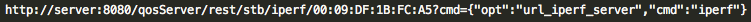
\includegraphics[width=\textwidth]{00_media/url_iperf}
      \caption{URL finale d'iperf pour Web Service}
      \label{gra:maqmenu}
\end{figure}